%===========================================================================%
% MECH 559 Project
% Khalil B. Al Handawi
%===========================================================================%
%Package definition

\documentclass[11pt]{article}

\usepackage[headsep=.2in,footskip=.2in]{geometry}
\geometry{
letterpaper,
total={215.9mm,279.4mm},
left=0.75in,
right=0.75in,
top=0.75in,
bottom=0.75in,
}

\usepackage[bookmarks=false]{hyperref} %hyperlinked cross-references
\hypersetup{
    colorlinks=true,
    linkcolor=blue,
    filecolor=magenta,      
    urlcolor=cyan,
    citecolor=blue,
}
\usepackage{booktabs}
\usepackage{titlesec} % title formatting package

% % section title spacing
% \titlespacing\section{0pt}{6pt plus 4pt minus 2pt}{4pt plus 2pt minus 2pt}
% \titlespacing\subsection{0pt}{6pt plus 4pt minus 2pt}{4pt plus 2pt minus 2pt}
% \titlespacing\subsubsection{0pt}{6pt plus 4pt minus 2pt}{4pt plus 2pt minus 2pt} 

% \titleformat{\section}
% {\normalsize\bfseries}
% {\thesection.}{0.5em}{} % section formatting

% \titleformat{\subsubsection}
% {\normalsize\itshape}
% {\thesubsubsection}{0.5em}{} % subsubsection formatting

% \setlength\parindent{2pt} % no paragraph indentation

\usepackage{array} % for \arraybackslash command
\usepackage{color}

\usepackage{graphicx} % To import graphics
\graphicspath{ {images/} }
\usepackage[font=normalsize,skip=0pt]{caption}
\usepackage{subcaption}
\usepackage{wrapfig} % Wrap figure
\usepackage{multirow}% tables

\usepackage{amsmath}
\usepackage{bm}
\usepackage{enumitem} % reduce bullet spacing
\usepackage{amssymb} % for mathbb symbols

% \usepackage{mathptmx}
% \usepackage[T1]{fontenc} % for nimbus roman font
\usepackage[french,british]{babel}

% Reduce spacing between bibliographic items
\let\OLDthebibliography\thebibliography
\renewcommand\thebibliography[1]{
  \OLDthebibliography{#1}
  \setlength{\parskip}{0pt}
  \setlength{\itemsep}{0pt plus 0.3ex}
}

\usepackage{fancyhdr}
\renewcommand{\headrulewidth}{0pt} % remove top header line
\pagestyle{fancy}
\cfoot{\thepage}

\newcolumntype{C}[1]{>{\centering\arraybackslash}p{#1}}
\newcolumntype{L}[1]{>{\arraybackslash}p{#1}}
\newcolumntype{R}[1]{>{\flushright\arraybackslash}p{#1}}
\newcommand{\mc}[1]{\multicolumn{1}{c}{#1}} % multicolumn command

% new commands
\newcommand{\coursenumber}{MECH559}
\newcommand{\projecttitle}{Design of a supersonic business jet}
\newcommand{\semester}{Fall 2021}
\newcommand{\professor}{Prof. Michael Kokkolaras}

%========================= ACRONYMS ================================%
\usepackage{acro}
\DeclareAcronym{MDO}{ short = MDO, long = multidisciplinary design optimization, short-plural = s, long-plural = s}
\DeclareAcronym{MADS}{ short = MADS, long = mesh adaptive direct search, short-plural = s, long-plural = s}
\DeclareAcronym{ATC}{ short = ATC, long = analytical target cascading, short-plural = s, long-plural = s}
\DeclareAcronym{SBJ}{ short = SBJ, long = supersonic business jet, short-plural = s, long-plural = s}
%=================================================================%

%%%%%%%%%%%%%%%%%%%%%%%%%%%%%%%%%%%%%%%%%%%%%%%%%%%%%%%%%%%%%%%%%%%%%%
\begin{document}

% a) the problem, b) the theoretical approach, c) the objectives, d) the methodology or approach used (avoid abbreviations)

\restoregeometry
\pagenumbering{roman}

\newpage
\pagenumbering{arabic}

%======================== PROBLEM DESCRIPTION ========================%
\cleardoublepage

\rhead{\projecttitle}
\lhead{\coursenumber, \semester}
\setcounter{page}{1}

%%%%%%%%%%%%%%%%%%%%%%%%%%%%%%%%%%%%%%%%%%%%%%%%%%%%%
\section*{Design of a supersonic business jet} \label{sec:intro}

A \ac{SBJ} design problem is used to demonstrate different \ac{ATC} formulations used for solving design problems involving multiple disciplines. The supersonic business jet design problem involves four subproblems; An overall \textbf{aircraft}, \textbf{propulsion}, \textbf{aerodynamics}, and \textbf{structural} design subproblems.

The \texttt{MATLAB} code that describes the inputs, outputs and underlying analyses for each subproblem is provided in the \texttt{NoHiMDO} code repository on \texttt{myCourses} inside the folder \texttt{SBJ}.

The individual \texttt{MATLAB} files for each subanalysis and their inputs and outputs are given in Table~\ref{table:subproblem}. The definition for each input and output is given in Table~\ref{table:parameters}.

Based on these definitions, two possible formulations for a \ac{MDO} problem are provided. The objective is to minimize the total weight of the aircraft $W_t$ given by subproblem 1. 

Figure~\ref{fig:uncoupled} describes an \ac{ATC} formulation where subproblem 1 coordinates the solutions to the other 3 subproblems. There is no direct coupling between the individual subproblems. This is an example of a hierarchal \ac{ATC} formulation.

Figure~\ref{fig:coupled} describes an \ac{ATC} formulation where the relevant inputs and outputs of each subproblem are directly coupled. This is an example of a non-hierarchal \ac{ATC} formulation.

\begin{table}[h!]
  \centering
  \renewcommand{\arraystretch}{1.0}% Wider
  \small\addtolength{\tabcolsep}{-1pt}
  \caption{Supersonic business jet subproblem definitions}
  \label{table:subproblem}
  \begin{tabular}{L{2cm}C{1cm}C{4cm}C{4cm}R{5cm}}
    \hline\hline
    \bf Subproblem          & \bf number  & \bf Inputs                                                                                                                                                      & \bf Output                                                      & \bf \texttt{MATLAB} file              \\ \hline
    Aircraft                & 1           & $W_e$, $W_f$, $W_s$, $h$, $M$, $L/D$, $\text{SFC}$                                                                                                              & $W_t$, $\text{range}$     		                                  & \texttt{SBJ\_analysis\_range.m}       \\ \hline
    Propulsion 	            & 2           & $h$, $M$, $T$, $D$                                                                                                                                              & $\text{SFC}$, $W_e$, $\text{ESF}$, $T_{E}$, $\text{Throttle}$   & \texttt{SBJ\_analysis\_power.m}       \\ \hline
    Aerodynamics 	          & 3           & $t/c$, $h$, $M$, $AR_w$, $\Lambda_w$, $S_\text{ref}$, $S_\text{ht}$, $AR_\text{ht}$, $\Lambda_\text{ht}$, $L_w$, $L_\text{ht}$, $W_t$, $\theta$, $\text{ESF}$   & $L$, $D$, $L/D$, $P_g$, $CLo_1$, $CLo_2$                        & \texttt{SBJ\_analysis\_dragpolar.m}   \\ \hline
    Structures 		          & 4           & $t/c$, $h$, $M$, $AR_w$, $\Lambda_w$, $S_\text{ref}$, $S_\text{ht}$, $AR_\text{ht}$, $\mathbf{t}$, $\mathbf{t}_s$, $\lambda$, $L$                               & $W_s$, $W_f$, $\theta$, $\mathbf{g}_1$                          & \texttt{SBJ\_analysis\_structural.m}  \\ 
    \hline\hline  
  \end{tabular}
\end{table}

\begin{figure}[h!]
	\centering
	\subfloat[\label{fig:uncoupled} \ac{ATC} Formulation 1 (Hierarchical)]{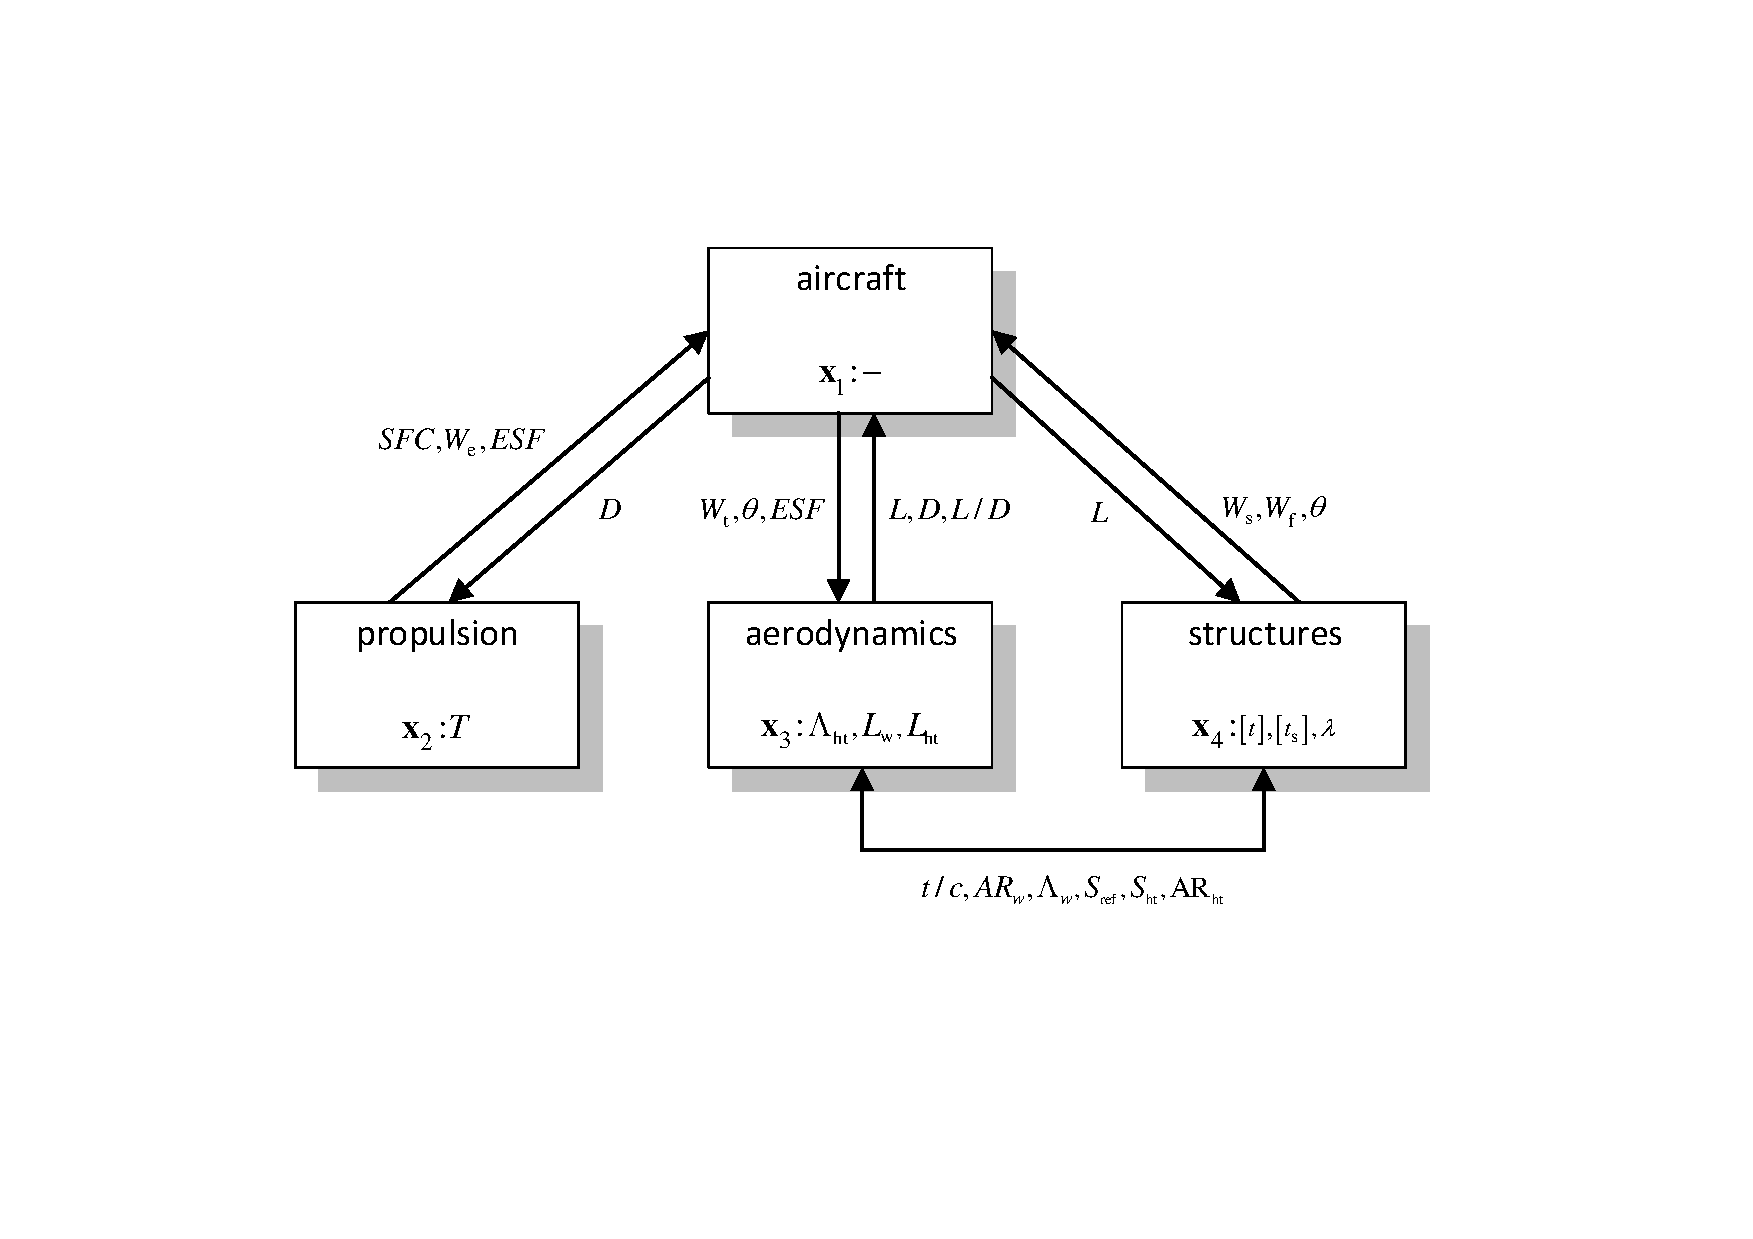
\includegraphics[width=0.5\textwidth]{MDO_schematics_1.pdf}}
  \subfloat[\label{fig:coupled} \ac{ATC} Formulation 2 (Non-hierarchical)]{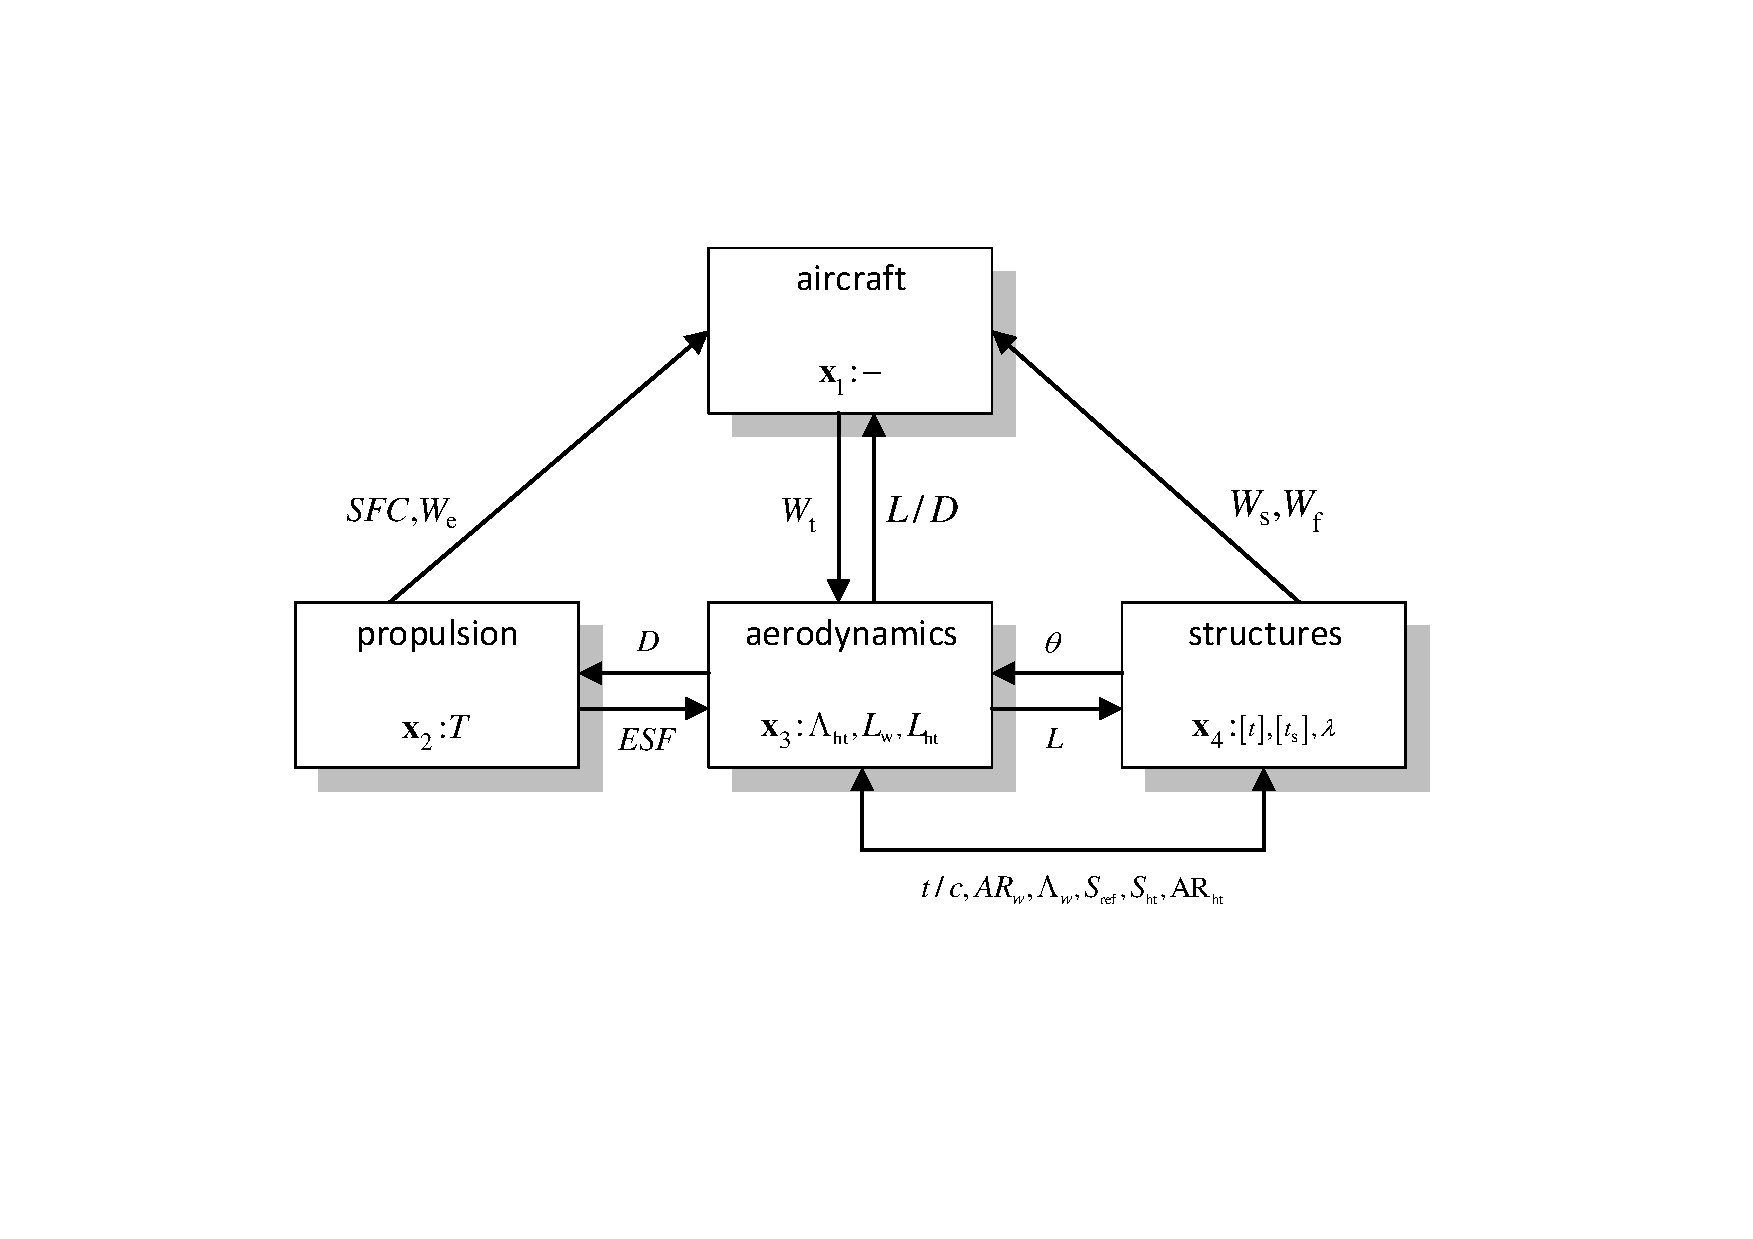
\includegraphics[width=0.5\textwidth]{MDO_schematics_2.pdf}}
  \caption[]{ATC formulation of \ac{SBJ} problem}
\end{figure}

\begin{table}[h!]
  \centering
  \renewcommand{\arraystretch}{1.0}% Wider
  \small\addtolength{\tabcolsep}{-1pt}
  \caption{Supersonic business jet design variables}
  \label{table:parameters}
  \begin{tabular}{lcccr}
    \hline\hline
    \bf Variable            & \bf code designation  & \bf lower bound & \bf upper bound & \bf description           \\ \hline
    $t/c$                   & \texttt{tc}           & 0.01      	 		& 0.1     		    & Thickness/chord           \\
    $AR_{\text{w}}$ 	      & \texttt{ARw}          & 2.5             & 8         	    & Wing aspect ratio         \\
    $\Lambda_{\text{w}}$ 		& \texttt{LAMBDAw}      & 40					    & 70    	  	    & Wing sweep angle          \\
    $S_{\text{ref}}$ 	      & \texttt{Sref}         & 200					    & 800   	  	    & Wing surface area         \\
    $S_{\text{ht}}$ 			  & \texttt{Sht}          & 50				      & 148.9		  	    & Tail surface area         \\
    $AR_{\text{ht}}$  			& \texttt{ARht}         & 2.5			        & 8.5   	  	    & Tail aspect ratio         \\
    $T$ 				            & \texttt{T}            & 0.1		 			    & 1.0    		      & Thrust                    \\
    $\Lambda_\text{ht}$ 	  & \texttt{LAMBDAht}     & 40              & 70    		  	  & Tail sweep                \\
    $L_{\text{w}}$ 				  & \texttt{Lw}           & 0.01            & 0.2    		      & Wing distance             \\
    $L_{\text{ht}}$ 				& \texttt{Lht}          & 1               & 3.5    		      & Tail distance             \\
    $\mathbf{t}$ 			      & \texttt{t}            & 0.1             & 4.0    		      & Nine thicknesses          \\
    $\mathbf{t}_{\text{s}}$ & \texttt{ts}           & 0.1             & 9.0    		      & Nine thicknesses          \\
    $\lambda$ 	            & \texttt{lambda}       & 0.1             & 0.4    		  	  & Taper ratio               \\
    $L$ 				            & \texttt{L}            & 5000            & 100000    		  & Total lift                \\
    $W_{\text{e}}$ 			    & \texttt{We}           & 100             & 30000  		      & Engine weight             \\
    $W_{\text{t}}$		      & \texttt{Wt}           & 5000            & 100000    		  & Total weight              \\
    $\theta$ 		            & \texttt{theta}        & 0.2             & 50    		  	  & Wing twist                \\
    ESF 		                & \texttt{ESF}          & 0.5             & 1.5    		  	  & Engine scaling factor     \\
    $D$ 		                & \texttt{D}            & 1000            & 70000	  	      & Total drag                \\
    $W_{\text{f}}$ 		      & \texttt{Wf}           & 5000            & 100000    		  & Fuel weight               \\
    $L/D$ 		              & \texttt{LD}           & 0.1             & 10    		  	  & Lift/drag ratio           \\
    SFC 		                & \texttt{SFC}          & 1               & 4    		  	    & Specific fuel consumption \\
    $W_{\text{s}}$ 		      & \texttt{Ws}           & 5000            & 100000    		  & Structural weight         \\ \hline
    \multicolumn{5}{c}{\bf Used for defining constraints}                                                           \\ \hline
    range 		              & \texttt{range}        &                 &            		  & Aircraft range            \\
    $T_{\text{E}}$ 		      & \texttt{Temp\_E}      &                 &            		  & Engine temperature        \\
    Throttle 		            & \texttt{Throttle\_uA} &                 &            		  & Engine throttle setting   \\
    $P_{\text{g}}$ 		      & \texttt{Pg}           &                 &            		  & Pressure gradient         \\
    $CLo_{1}$ 		          & \texttt{CLo1}         &                 &            		  & Lift coefficient 1        \\
    $CLo_{2}$ 		          & \texttt{CLo2}         &                 &            		  & Lift coefficient 2        \\
    $\mathbf{g}_1$ 		      & \texttt{G1}           &                 &            		  & Structural constraints    \\ \hline
    \multicolumn{5}{c}{\bf Constants}                                                                               \\ \hline
    $M$ 		                & \texttt{M}            & \multicolumn{2}{c}{1.4}           & Aircraft mach number      \\
    $h$ 		                & \texttt{h}            & \multicolumn{2}{c}{55000}         & Cruising altitude         \\
    \hline\hline
  \end{tabular}
\end{table}

\newpage
%%%%%%%%%%%%%%%%%%%%%%%%%%%%%%%%%%%%%%%%%%%%%%%%%%%%%
\section*{Project deliverables} \label{sec:intro}

\begin{table}[h!]
  \centering
  \renewcommand{\arraystretch}{1.2}% Wider
  \small\addtolength{\tabcolsep}{1pt}
  \caption{\texttt{NoHiMDO} algorithmic parameters}
  \label{table:algoparameters}
  \begin{tabular}{lc>{\centering\arraybackslash}p{5.5cm}>{\centering\arraybackslash}p{6cm}}
    \hline\hline
    \bf Parameter               & \bf Default & \bf Possible values               & \bf Description                                                               \\ \hline
    \texttt{display}            & true        & true,false                        & verbosity                                                                     \\
    \texttt{w\_scheme}          & 'median'    & 'median','max','normal','rank'    & Update scheme                                                                 \\
    \texttt{constraints\_cv}    & true				& true,false				                & Penalty if coupling variables out of bounds                                   \\
    \texttt{realistic\_obj}     & false				& true,false				                & Realistic objective                                                           \\
    \texttt{inc\_stop}          & 1e-12				&	real number $> 0$			            & Algo stops if this inconsistency is reached                                   \\
    \texttt{tol}                & 1e-12			  & real number $> 0$			            & Stop criteria on psize                                                        \\
    \texttt{noprogress\_stop}   & 100		 			& integer $> 1$		 			            & Algo stops if the inconsistency has not decreased this number of iterations   \\
    \texttt{NI}                 & 100         & integer $> 1$                     & Number of inner loop iterations                                               \\
    \texttt{NO}                 & 100         & integer $> 1$                     & Number of outer loop iterations                                               \\
    \texttt{beta}               & 2           & real number $> 0$                 & Hyper-parameter of the penalty update scheme                                  \\
    \texttt{gamma}              & 0.5         & real number $> 0$                 & Hyper-parameter of the penalty update scheme                                  \\
    \texttt{w0}                 & 1           & real number $> 0, < 1$            & Initial value for the w vector                                                \\
    \texttt{x0}                 & []          & vector of real numbers $> 0, < 1$ & Initial design                                                                \\
    \texttt{nb\_proc}           & 1           & integer $> 0$                     & Number of processors (requires \texttt{MATLAB} parallel computing toolbox)    \\
    \texttt{save\_subproblems}  & false       & true,false                        & Save detail of each subproblem                                                \\
    \texttt{solver}             & 'mads'      & 'mads','sqp','interior-point','active-set','trust-region-reflective' & Solver                                     \\
    \texttt{solver\_display}    & false       & true,false                        & Solver display                                                                \\

    \hline\hline
  \end{tabular}
\end{table}

\begin{enumerate}
  \item Execute the hierarchal \ac{ATC} formulation of the supersonic business jet problem by executing the matlab file \texttt{SBJ\_main.m}
  \begin{enumerate}
    \item Record the objective value $f$, and maximum inconsistency $\epsilon_q$.
    \item Take a screenshot of the figure showing the progress of optimization.
    \item Check \texttt{SBJ\_subsystem\_analysis\_1.m} and \texttt{SBJ\_problem\_definition\_1.m} located in the main directory. The comments and annotations here will help you understand how to define objectives, constraints, shared variables, and coupling variables for the \texttt{NoHiMOD} algorithm.
  \end{enumerate}
  \item Execute the non-hierarchal \ac{ATC} formulation of the supersonic business jet problem by uncommenting line 47 and commenting line 46 in \texttt{SBJ\_main.m}.
  \begin{enumerate}
    \item Record the objective value $f$, and maximum inconsistency $\epsilon_q$.
    \item Take a screenshot of the figure showing the progress of optimization.
  \end{enumerate}
  \item Comment on the difference in performance between the two formulations. Note and compare the number of iterations it took for the maximum inconsistency and objective values to stabilize.
  \item Based on your observations from solving the hierarchal and non-hierarchal problems, provide an analogy in terms of management style that you may have observed in the industry (during an internship) and describe which one is potentially more efficient for reducing lead times of complex engineering products.
  \item Formulate at least one more problem based on the supersonic business jet analyses.
  \begin{enumerate}
    \item Create a diagram showing the flow of the analysis variables between the different disciplines (similar to Figures~\ref{fig:uncoupled} and \ref{fig:coupled}).
    \item Mathematically express your formulation of the problem by writing down the optimization problems to be solved by each discipline (hint check the appendix of \cite{Tosserams2010,Talgorn2017a} for example formulations). Be sure to describe
    \begin{itemize}
      \item the objectives,
      \item constraints,
      \item variables to be optimized,
      \item and inconsistencies to be coordinated by the problem.
    \end{itemize}
    \item Define new \texttt{SBJ\_subsystem\_analysis\_x.m} and \texttt{SBJ\_problem\_definition\_x.m} files.
    \item Solve your problem using \texttt{NoHiMDO} by executing \texttt{SBJ\_main.m}
    \item Record the objective value $f$, and maximum inconsistency $\epsilon_q$.
    \item Take a screenshot of the figure showing the progress of optimization.
  \end{enumerate}
  \item Comment on the performance of your formulation of the problem relative to the hierarchal and non-hierarchal formulations.
  \item Adjust the algorithmic parameters of \texttt{NoHiMDO} given by Table~\ref{table:algoparameters} and solve all three (or more) formulations of the problem and comment on how the performance of the algorithm was affected by these changes. Select at least three parameters that you think are the most significant ones for improving the algorithm's performance.
\end{enumerate}

%========================= REFERENCES ================================%
\bibliographystyle{myIEEEtran}
\bibliography{MECH559_project_bibliography}

\end{document}